\documentclass{article}

\usepackage{geometry}
\usepackage{graphicx}

\setlength{\parindent}{0pt}
\setlength{\parskip}{5pt}

\title{CORE111 Logical Problem Solving\\Homework 5}
\author{My Name}

\begin{document}
\maketitle

\section{Translating into predicate logic form}

Assuming the predicates used are unambiguous, the definition of predicates have not been given.

(a) $\exists x (E(x) \wedge G(x)) \iff \exists y (M(y) \wedge G(y)) $

(b) $\forall x \forall y (((x \neq y) \wedge S(x,y)) \rightarrow (O(x,y) \vee O(y,x)) \wedge \neg (O(x,y) \wedge O(y,x)))$

(c) $\exists x (GGF(x) \wedge I(x,B))$

(d) $\forall x ((A(x) \wedge E(x) \wedge P(x) \wedge F(x)) \rightarrow (x=F.D.R)) $

(e) $\neg \exists x (H(x) \wedge F(x))$

(f) $\forall x (D(x) \rightarrow \neg P(x))$

(g) $\exists x (C(x) \wedge \neg B(x) \wedge \neg S(x)$

(h) $\forall x (H(x) \rightarrow S(x))$ (H(x) : x is a human)

(i) $\forall x (P(x) \rightarrow S(x)) \wedge \forall y (V(y) \rightarrow L(y))$

(j) $\exists x \exists y ((x \neq y) \wedge C(x) \wedge C(y) \wedge \forall z (C(z) \rightarrow (z=x \vee z=y)\wedge \neg (z=x \wedge z=y))$

\section{Proofs}

(a) 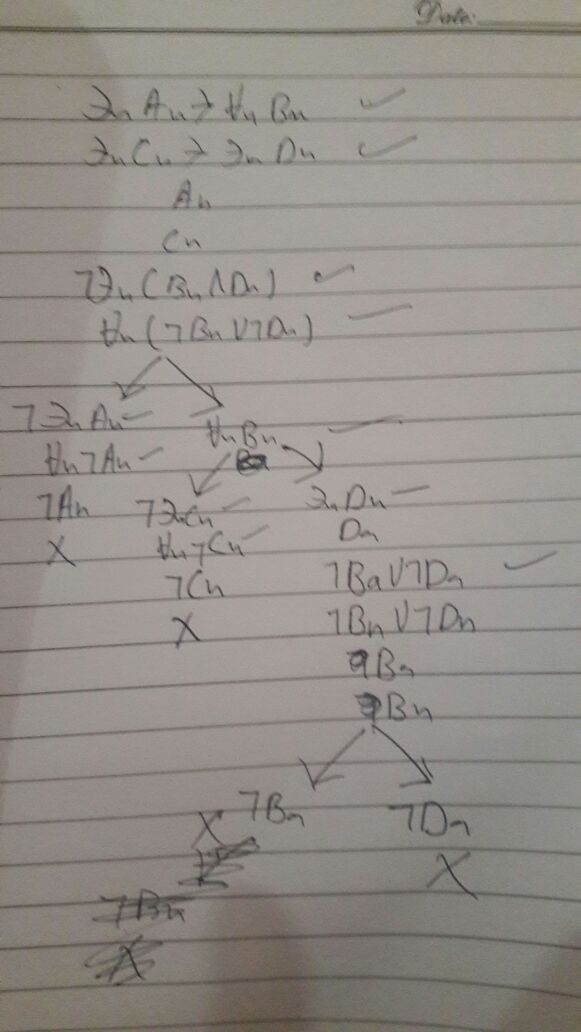
\includegraphics[width=\linewidth]{IMG_1018.JPG}

(b) 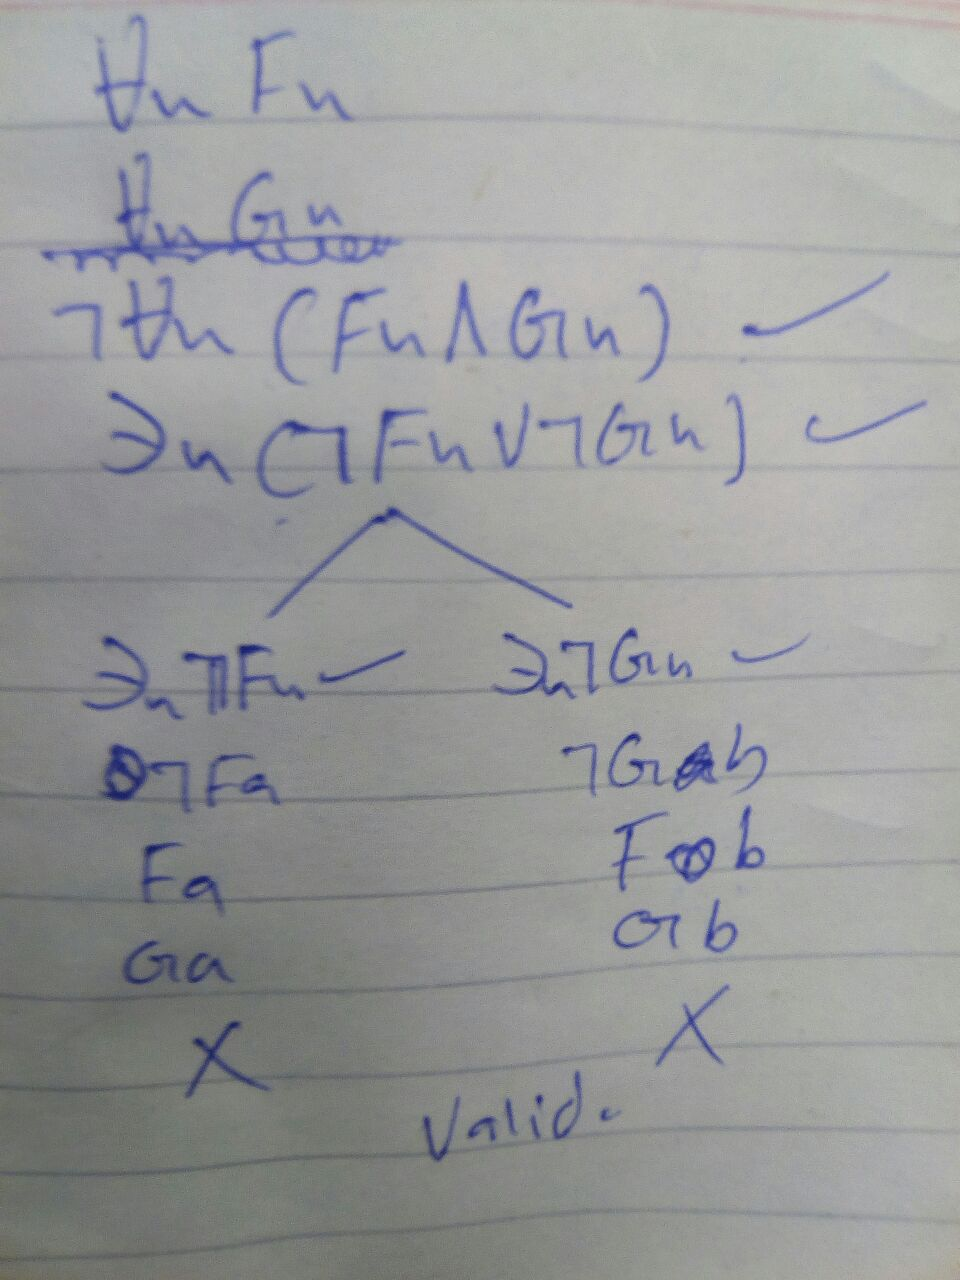
\includegraphics[width=\linewidth]{IMG_1023.JPG}

(c) 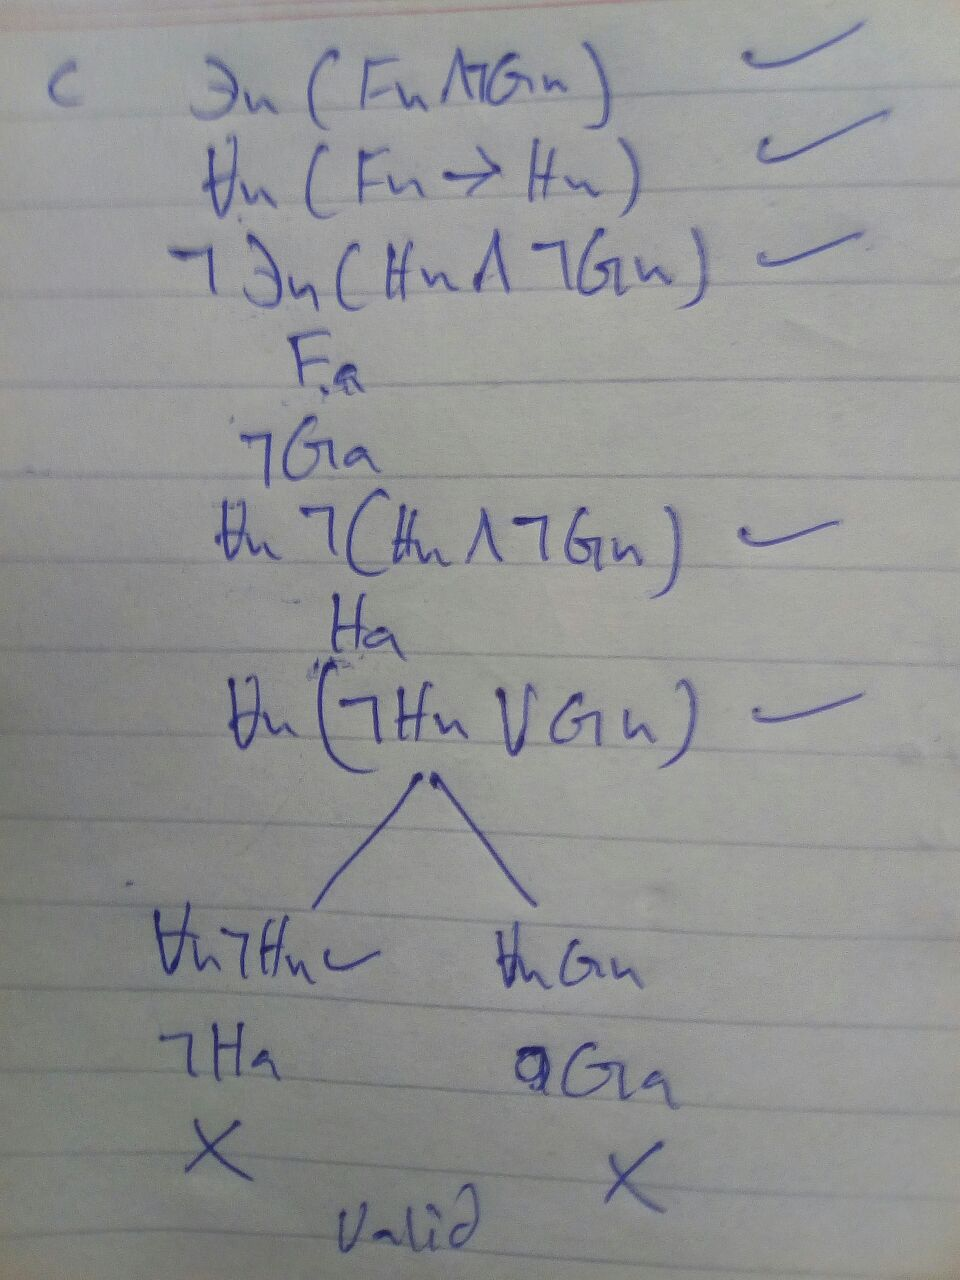
\includegraphics[width=\linewidth]{IMG_1022.JPG}

(d) 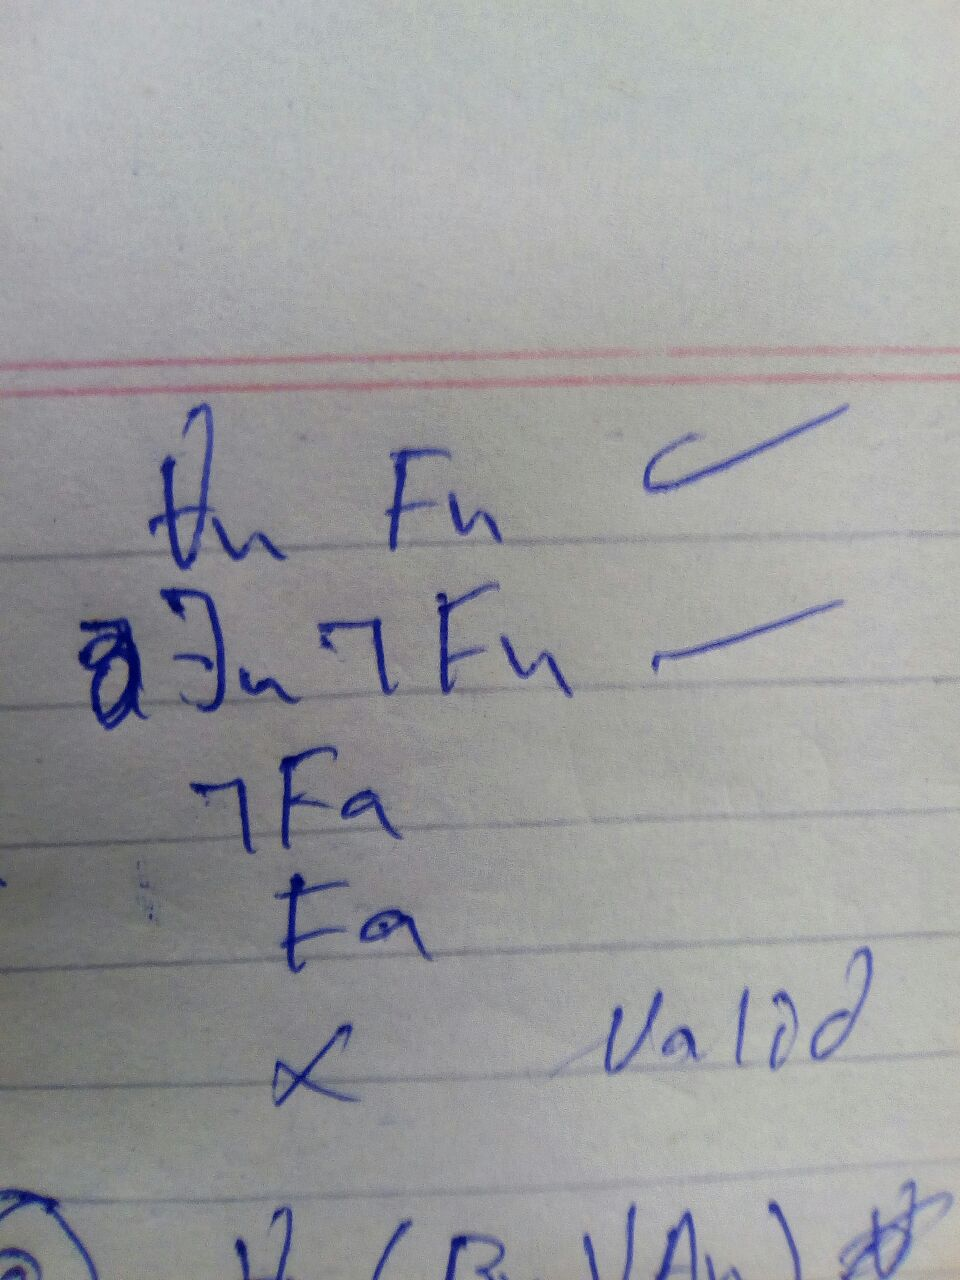
\includegraphics[width=\linewidth]{IMG_1021.JPG}

(e) 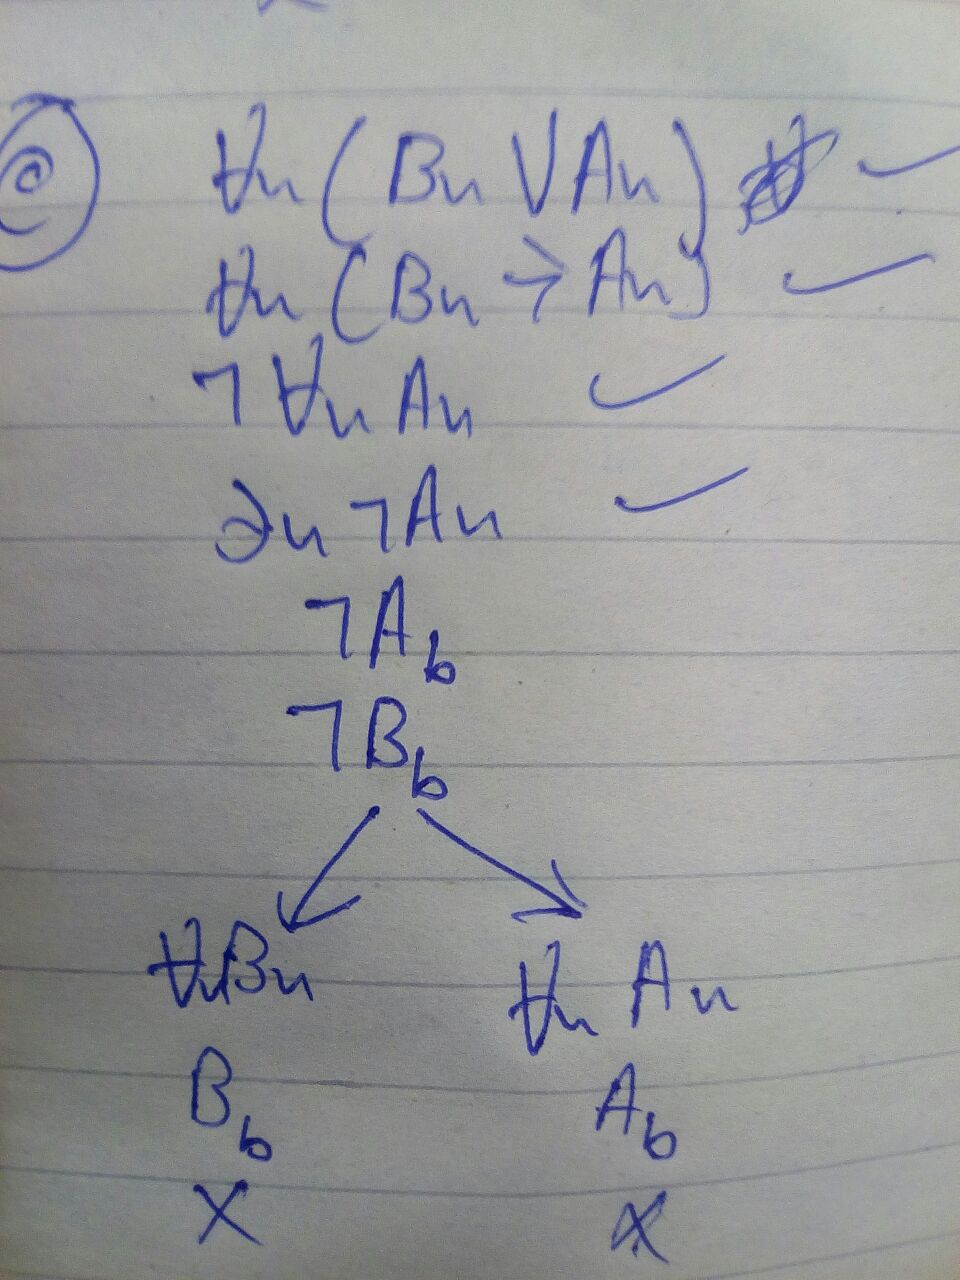
\includegraphics[width=\linewidth]{IMG_1020.JPG}

\end{document}